\documentclass[10pt,twocolumn]{article}
\usepackage[utf8]{inputenc}
\usepackage[T1]{fontenc}
\usepackage[english]{babel}
\usepackage[margin=1.55cm,columnsep=.62cm]{geometry}
\usepackage{lmodern,microtype,amsmath,amssymb,graphicx,subcaption}
\usepackage{booktabs,tabularx,array,enumitem,xcolor,hyperref,url,caption}
\graphicspath{{Documentation/images/}}
\hypersetup{colorlinks=true,urlcolor=blue!55!black,linkcolor=blue!50!black,pdftitle={LMT calibration project report}}
\setlist{nosep,leftmargin=*}
\captionsetup{font=small,labelfont=bf}
\sloppy
\title{\textbf{Logistic Model Trees for Probabilistic Calibration}\\\large Research project overview and experimental findings}
\author{Allison Lara Nieva\\\small MITACS Globalink Research Internship, Université du Québec à Montréal (UQAM)\\\small Project 45286: Combining Decision Trees and Regression Models}
\date{June--August 2025}
\begin{document}
\maketitle
\begin{abstract}
This report reconstructs the LMT-calibration project from its public repository, emphasizing the Documentation folder and commit chronology. The work implemented Logistic Model Trees (LMTs), assessed probability calibration, and explored alternative tree growth and pruning. It progressed from initial LMT implementation to synthetic calibration experiments and a final linear-spline tree. The repository reports qualitative comparisons but no consolidated numeric results table; conclusions are limited to what its documentation supports.
\end{abstract}
\section{Project aim and working hypothesis}
Decision trees represent nonlinear patterns, but probability estimates can be piecewise constant. Logistic regression gives probabilities, but a single global model may be too restrictive. An LMT combines tree-based partitioning with local logistic models trained using LogitBoost to produce probabilities in different regions of feature space \cite{landwehr}.

The project asked whether this combination could retain nonlinear flexibility while improving probability quality. The repository does not state a separately preregistered hypothesis. The working hypothesis can be reconstructed as follows: local logistic models within a tree may give more informative probabilities than a plain tree, while calibration-sensitive split and pruning criteria may improve calibration without a large loss in discrimination. This is an interpretation of the documented goal, not a verbatim or confirmed claim.
\section{Initial approach}
The first stage implemented the original LMT framework of Landwehr, Hall, and Frank. An entropy-based tree partitions the data; LogitBoost fits logistic models on observations reaching nodes or leaves. Cross-validation selects boosting iterations. In the faster LMT V2 implementation, the root selects the number of rounds and child models warm-start from their parent.

The initial checks examined predictions, decision regions, probability surfaces, and probability histograms. Comparisons with plain trees and logistic baselines used accuracy, ROC-AUC, Brier score, log loss, and calibration curves. Commit history records that pruning was missing from the first implementation; it was completed before the broader dataset tests.
\begin{figure}[t]\centering
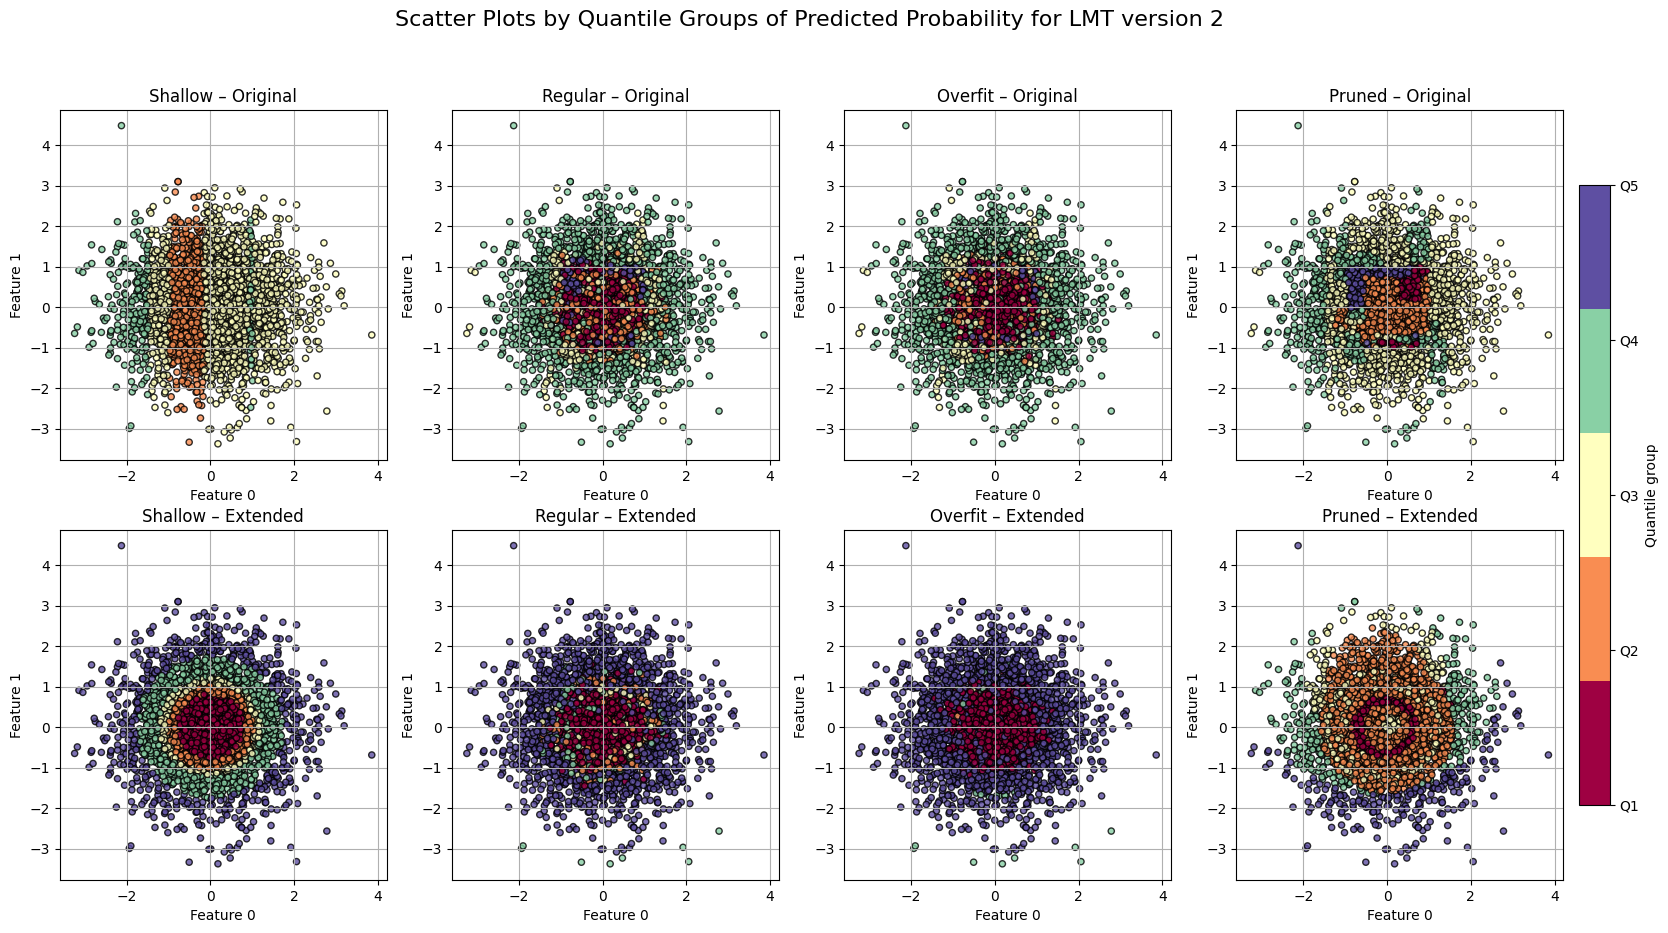
\includegraphics[width=.96\columnwidth]{scatter.png}
\caption{Test cases grouped by predicted-probability quintile for an original LMT.}\label{fig:scatter}
\end{figure}

\section{Datasets and calibration}
Synthetic data with known probabilities allowed direct calibration evaluation. Features $X_1,X_2$ were independent standard normal variables and labels were drawn from a Bernoulli distribution with a logistic probability. In the circle generator, the score depended on squared distance from the origin. In the diamond generator, it depended on $|X_1|+|X_2|$. The final MVP used $n=5{,}000$, $\alpha=2$, and $r_0=1.5$.

Other tests used clean and noisy make-circles data, two- and three-class spirals, and the Breast Cancer Wisconsin dataset supplied by scikit-learn. These covered curved boundaries, noise sensitivity, multiclass prediction, and an initial real-data sanity check.

\begin{figure}[t]\centering
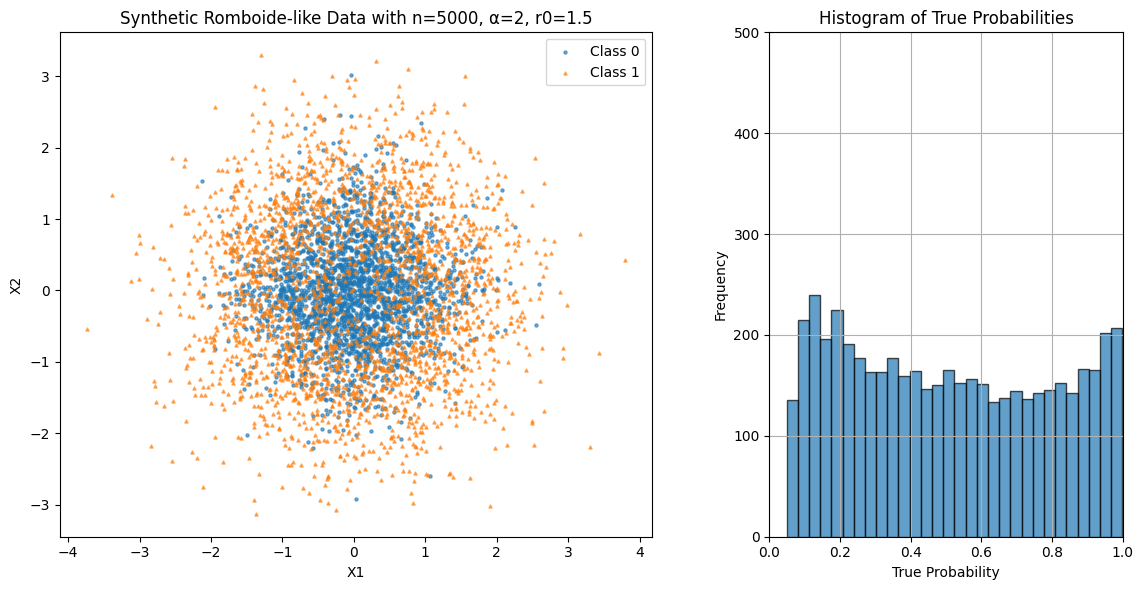
\includegraphics[width=.96\columnwidth]{dgp_absolute.png}
\caption{Absolute-value data-generating process with a diamond-shaped probability boundary.}\label{fig:dgp}
\end{figure}

Accuracy and ROC-AUC assess classification and ranking; Brier score and log loss assess probabilistic accuracy. Expected Calibration Error and reliability diagrams compare predicted probability with observed frequency. When the true probability is known, the notebooks also compare predictions against ground truth using true-probability Brier and log loss, reducing noise from sampled binary labels \cite{gruber,machado}.

\section{Later experiments: splitting and pruning}
\textbf{AUC-threshold and cost-complexity pruning.} Permissive trees were simplified using breadth-first node-wise AUC-threshold pruning or scikit-learn cost-complexity pruning. Diamond and circle experiments compared tree size, decision regions, and basic accuracy/AUC. The documentation explicitly says Brier score, log loss, and ECE were not computed in this suite; it cannot establish calibration superiority.

\textbf{Root multi-cuts.} An exploratory alternative selected multiple thresholds at the root and fitted a separate tree in each resulting region, optionally adding LMT models. The repository README reports poor performance, so this approach was not selected as final.
\textbf{Linear-spline tree.} The later method tested candidate feature and knot pairs $(X_j,\tau)$. At a node, a logistic model used the basis $\{1,X_j,(X_j-\tau)_+\}$, where $(z)_+=\max(0,z)$. A hard split at the knot created two children. One criterion maximized size-weighted child AUC; another minimized size-weighted child Brier score. Minimum child size, maximum depth, and purity rules constrained growth.

\textbf{Regression pruning.} After growth, LogitBoost models could be attached to nodes. The original rule collapsed descendants when a node's own AUC passed threshold $\delta$. Local-gain pruning retained a split only when the children's size-weighted AUC improved on the parent by at least $\delta$. Cross-validation selected $\delta$ using Brier score or log loss, so the pruning measure (AUC) could differ from the objective used to choose pruning strength.

\begin{figure*}[t]\centering
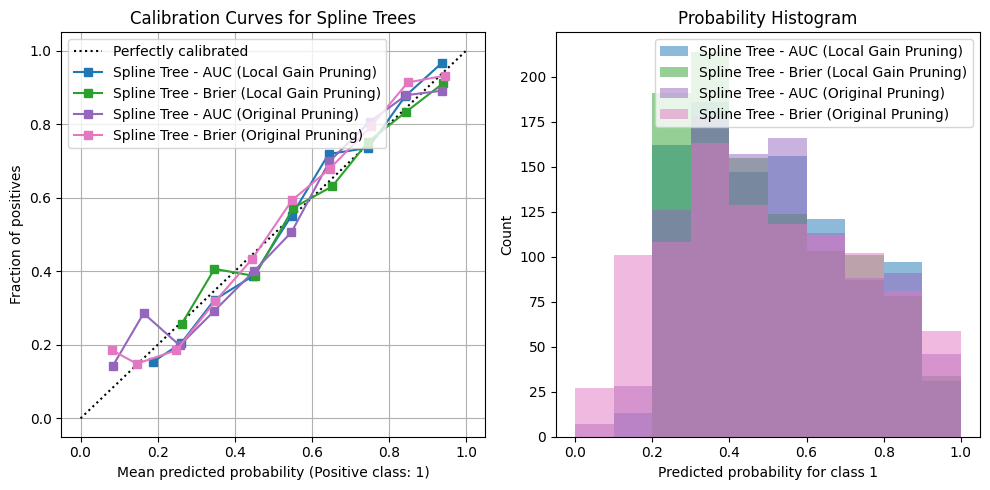
\includegraphics[width=.47\textwidth]{calibration_pruned.png}\hfill
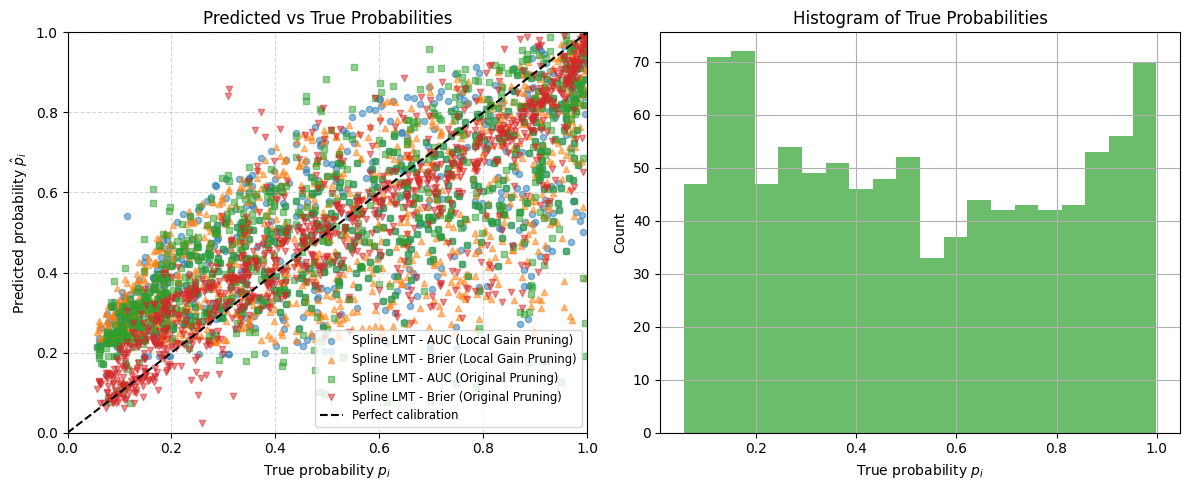
\includegraphics[width=.47\textwidth]{true_pruned.png}
\caption{Final MVP calibration diagnostics: reliability curves (left) and true versus predicted probabilities (right). The diagonal indicates ideal agreement.}\label{fig:mvp}
\end{figure*}

\section{Results by experiment}
\begin{table*}[t]\centering\small
\caption{Findings reported in the repository documentation.}
\begin{tabularx}{\textwidth}{@{}p{.23\textwidth}p{.32\textwidth}X@{}}
\toprule
\textbf{Stage} & \textbf{Comparison} & \textbf{Reported finding}\\
\midrule
Original LMT & LMT and plain-tree/logistic baselines on synthetic and Breast Cancer data. & Established implementation and diagnostics. Guides list metrics and figures but do not consolidate numbers or claim uniform superiority.\\
Known-probability calibration & Tree/LMT configurations and original versus extended features. & Enabled direct comparison with ground truth. No single numeric summary is given in the documentation.\\
AUC pruning versus CCP & Tree size and boundaries on diamond and circle data. & Compared simplification; calibration losses were not computed in this set.\\
Root multi-cuts & Multiple root thresholds followed by regional trees. & Repository overview reports poor performance; this alternative was dropped.\\
Linear-spline split metric & AUC-based versus Brier-based growth. & Similar structures and test performance; final methodology note judges Brier-based growth better overall.\\
LMT and pruning variants & Unpruned LMT; original versus local-gain pruning; delta chosen by Brier or log loss. & Adding LogitBoost to fully grown trees did not improve calibration-sensitive losses. Pruning produced similarly compact trees and nearly identical out-of-sample Brier and log loss; differences were small relative to cross-validation variability.\\
\bottomrule
\end{tabularx}\label{tab:results}
\end{table*}

The final comparison used a diamond generator with $n=5{,}000$, $\alpha=2$, and $r_0=1.5$. The documentation reports qualitative comparisons rather than exact scores; this report does not infer effect sizes from figures. It supports an experiment-specific preference for Brier-based growth, while pruning alternatives yielded very similar final losses.
\section{Commit chronology}
Dates are repository commit dates in UTC. Representative links show the progression:
\begin{itemize}
\item \textbf{June 10--12:} project papers and LMT explanation added; formulas corrected. \href{https://github.com/Allison-Lara18/LMT-calibration/commit/e136f45b47}{Commit}.
\item \textbf{June 19:} binary and multiclass LogitBoost and first LMT implementation; pruning incomplete. \href{https://github.com/Allison-Lara18/LMT-calibration/commit/1a5eb027a0}{Commit}.
\item \textbf{June 26:} LMT implementation completed; tests began on make-circles and Breast Cancer. \href{https://github.com/Allison-Lara18/LMT-calibration/commit/0ff5942bff}{Commit}.
\item \textbf{July 3--10:} noisy circles, spirals, known-probability generators, and probability visualizations. \href{https://github.com/Allison-Lara18/LMT-calibration/commit/5e6b062380}{July 3} and \href{https://github.com/Allison-Lara18/LMT-calibration/commit/d5ce219ec5}{July 10}.
\item \textbf{July 17--23:} AUC-based pruning and experimental root initialization, then linear-spline splitting with LMT V2. \href{https://github.com/Allison-Lara18/LMT-calibration/commit/c04028e58e}{July 17} and \href{https://github.com/Allison-Lara18/LMT-calibration/commit/25eee85254}{July 23}.
\item \textbf{July 30--August 8:} threshold sweeps, split metrics, and local-gain pruning. \href{https://github.com/Allison-Lara18/LMT-calibration/commit/8f7b23f4d9}{July 30} and \href{https://github.com/Allison-Lara18/LMT-calibration/commit/5ff2011113}{August 8}.
\item \textbf{August 15--26:} theory documentation, final guides, and feedback corrections. \href{https://github.com/Allison-Lara18/LMT-calibration/commit/fcc2264c61}{August 15} and \href{https://github.com/Allison-Lara18/LMT-calibration/commit/ecfb3f7e67}{August 26}.
\end{itemize}\section{Interpretation and conclusion}
The project produced reusable code and increasingly calibration-aware experiments. Its clearest contribution is methodological: split and pruning choices could be compared using ranking and probability-quality criteria while tracking model complexity. The clearest final comparison is synthetic and uses one documented generator configuration. Earlier experiments are summarized mainly in notebook guides, rather than a consolidated table of estimates and uncertainty intervals. Final pruning differences were small relative to cross-validation variability. The evidence supports a cautious preference for Brier-based growth in that experiment, not a general claim that LMTs or one pruning rule always calibrate better. Calibration should be measured directly rather than inferred from accuracy or AUC.\begin{thebibliography}{9}
\bibitem{landwehr} N. Landwehr, M. Hall, and E. Frank, "Logistic model trees," \emph{Machine Learning}, 59(1--2), 161--205, 2005. \href{https://doi.org/10.1007/s10994-005-0466-3}{doi}.
\bibitem{gruber} S. G. Gruber and F. Buettner, "Better uncertainty calibration via proper scores for classification and beyond," \emph{Advances in Neural Information Processing Systems}, 35, 627--640, 2022.
\bibitem{machado} A. F. Machado, A. Charpentier, and F. Fernandes, "From uncertainty to precision: Enhancing binary classifier performance through calibration," 2024, as cited in the project README.
\bibitem{repository} A. Lara Nieva, \emph{LMT-calibration}, MITACS research repository. \url{https://github.com/Allison-Lara18/LMT-calibration}. Documentation: \url{https://github.com/Allison-Lara18/LMT-calibration/tree/main/Documentation}.
\end{thebibliography}
\end{document}